\documentclass[11pt]{article}

\usepackage{hyperref}
\usepackage{amsmath}
\usepackage{enumerate}
\usepackage{tikz}
\usepackage{verbatim}
\usetikzlibrary{arrows}
\newcommand{\bigO}{\ensuremath{\mathcal{O}}}

\title{\textbf{Algoritmen en Complexiteit HW 4}}
\author{Jelte Fennema (10183159)\\
		Jaap Koetsier (10440615)\\
        Abe Wiersma (10433120)}
\date{6 maart 2014}

\begin{document}

\maketitle

\begin{enumerate}
    \item
        \begin{enumerate}
            \item
                Dit is de begin graaf zonder stroomvergrotende paden:\\
                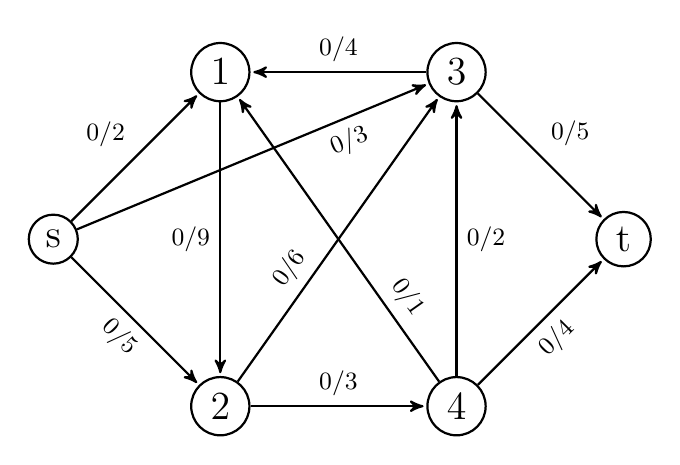
\begin{tikzpicture}[->,>=stealth',shorten >=1pt,auto,node distance=3cm,
                                    thick,main node/.style={circle,draw,font=\Large}]
                \node[main node] (S) {s};
                \node[main node] (1) [above right of=S] {1};
                \node[main node] (2) [below right of=S] {2};
                \node[main node] (3) [right of=1] {3};
                \node[main node] (4) [right of=2] {4};
                \node[main node] (T) [below right of=3] {t};
                \path[every node/.style={font=\small}]
                    (S)
                    edge node {0/2} (1)
                    edge node [below, sloped, pos=0.75]{0/3} (3)
                    edge node [below, sloped]{0/5} (2)

                    (1)
                    edge node [left] {0/9} (2)

                    (2)
                    edge node [sloped, pos=0.35] {0/6} (3)
                    edge node {0/3} (4)

                    (3)
                    edge node [above] {0/4} (1)
                    edge node {0/5} (T)

                    (4)
                    edge node [right] {0/2} (3)
                    edge node [below, sloped]{0/4} (T)
                    edge node [above, sloped, pos=.25] {0/1} (1);
                \end{tikzpicture}
                \\
                Om stroomvergrotende paden te vinden gebruiken we Dijkstra om
                het kortste pad qua aantal kanten te vinden. Een geheel gevulde
                kant wordt niet meer als kant gerekent.

                Het eerst gevonden stroomvergrotende pad is s, 3, t:

                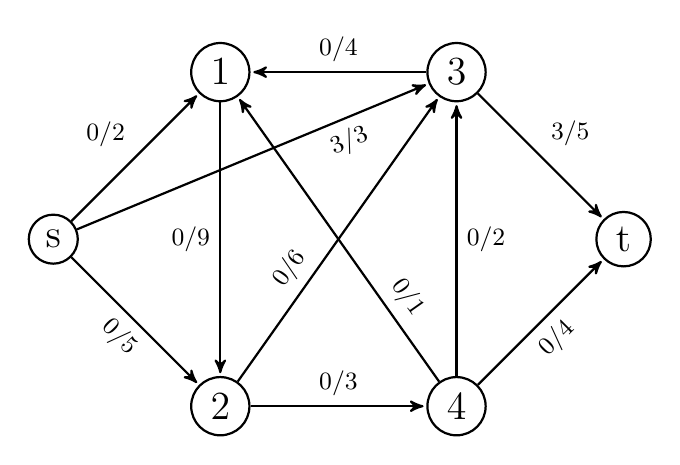
\begin{tikzpicture}[->,>=stealth',shorten >=1pt,auto,node distance=3cm,
                                    thick,main node/.style={circle,draw,font=\Large}]
                \node[main node] (S) {s};
                \node[main node] (1) [above right of=S] {1};
                \node[main node] (2) [below right of=S] {2};
                \node[main node] (3) [right of=1] {3};
                \node[main node] (4) [right of=2] {4};
                \node[main node] (T) [below right of=3] {t};
                \path[every node/.style={font=\small}]
                    (S)
                    edge node {0/2} (1)
                    edge node [below, sloped, pos=0.75]{3/3} (3)
                    edge node [below, sloped]{0/5} (2)

                    (1)
                    edge node [left] {0/9} (2)

                    (2)
                    edge node [sloped, pos=0.35] {0/6} (3)
                    edge node {0/3} (4)

                    (3)
                    edge node [above] {0/4} (1)
                    edge node {3/5} (T)

                    (4)
                    edge node [right] {0/2} (3)
                    edge node [below, sloped]{0/4} (T)
                    edge node [above, sloped, pos=.25] {0/1} (1);
                \end{tikzpicture}
                \\

                Het eerst volgende gevonden stroomvergrotende pad is s, 2, 4,
                t:\\

                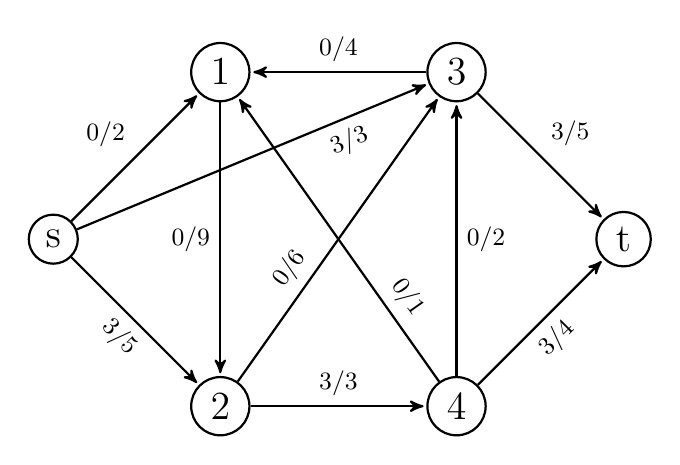
\begin{tikzpicture}[->,>=stealth',shorten >=1pt,auto,node distance=3cm,
                                    thick,main node/.style={circle,draw,font=\Large}]
                \node[main node] (S) {s};
                \node[main node] (1) [above right of=S] {1};
                \node[main node] (2) [below right of=S] {2};
                \node[main node] (3) [right of=1] {3};
                \node[main node] (4) [right of=2] {4};
                \node[main node] (T) [below right of=3] {t};
                \path[every node/.style={font=\small}]
                    (S)
                    edge node {0/2} (1)
                    edge node [below, sloped, pos=0.75]{3/3} (3)
                    edge node [below, sloped]{3/5} (2)

                    (1)
                    edge node [left] {0/9} (2)

                    (2)
                    edge node [sloped, pos=0.35] {0/6} (3)
                    edge node {3/3} (4)

                    (3)
                    edge node [above] {0/4} (1)
                    edge node {3/5} (T)

                    (4)
                    edge node [right] {0/2} (3)
                    edge node [below, sloped]{3/4} (T)
                    edge node [above, sloped, pos=.25] {0/1} (1);
                \end{tikzpicture}
                \\

                Het laatste gevonden stroomvergrotende pad is s, 2, 3, t:\\

                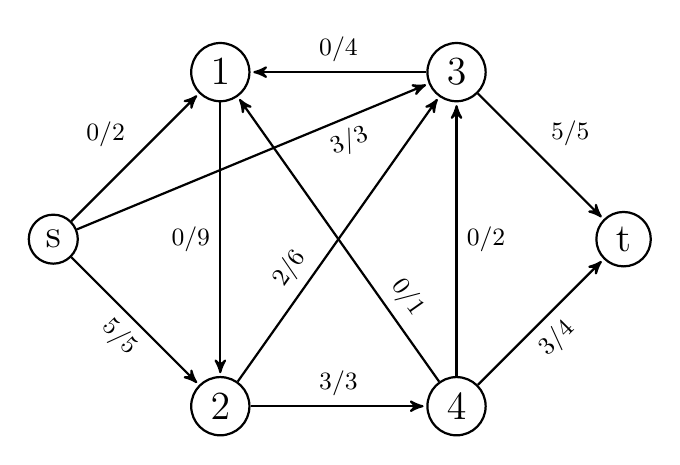
\begin{tikzpicture}[->,>=stealth',shorten >=1pt,auto,node distance=3cm,
                                    thick,main node/.style={circle,draw,font=\Large}]
                    \node[main node] (S) {s};
                    \node[main node] (1) [above right of=S] {1};
                    \node[main node] (2) [below right of=S] {2};
                    \node[main node] (3) [right of=1] {3};
                    \node[main node] (4) [right of=2] {4};
                    \node[main node] (T) [below right of=3] {t};
                    \path[every node/.style={font=\small}]
                        (S)
                        edge node {0/2} (1)
                        edge node [below, sloped, pos=0.75]{3/3} (3)
                        edge node [below, sloped]{5/5} (2)

                        (1)
                        edge node [left] {0/9} (2)

                        (2)
                        edge node [sloped, pos=0.35] {2/6} (3)
                        edge node {3/3} (4)

                        (3)
                        edge node [above] {0/4} (1)
                        edge node {5/5} (T)

                        (4)
                        edge node [right] {0/2} (3)
                        edge node [below, sloped]{3/4} (T)
                        edge node [above, sloped, pos=.25] {0/1} (1);
                \end{tikzpicture}
                \\

            \item
                Het gelaagde netwerk:\\
                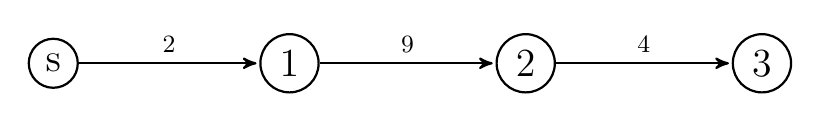
\begin{tikzpicture}[->,>=stealth',shorten >=1pt,auto,node distance=3cm,
                                    thick,main node/.style={circle,draw,font=\Large}]
                    \node[main node] (S) {s};
                    \node[main node] (1) [right of=S] {1};
                    \node[main node] (2) [right of=1] {2};
                    \node[main node] (3) [right of=2] {3};
                    \path[every node/.style={font=\small}]
                        (S)
                        edge node {2} (1)

                        (1)
                        edge node {9} (2)

                        (2)
                        edge node {4} (3)

                        ;
                \end{tikzpicture}


            \item

        \end{enumerate}

    \item

    \item
        \begin{enumerate}
            \item

            \item

            \item

        \end{enumerate}

    \item

\end{enumerate}

\end{document}
